% \vspace{-0.2cm}
\section{Broader Evaluation}
\label{sec:scaling_exp}


% \textbf{Experimental Setting:} 
We conduct large-scale experiments to further validate our methods. We train on a filtered subset of DAPO-Math~\citep{li2026optimal}, containing approximately 13k samples. Five model configurations (different base models and training techniques) are evaluated: (1) \textbf{MoE Base}: Qwen3-30B-A3B-Base~\citep{yang2025qwen3}; (2) \textbf{MoE Base w/ R3}: Qwen3-30B-A3B-Base with rollout router replay (R3)~\citep{ma2025stabilizing}; (3) \textbf{MoE Thinking}: Qwen3-30B-A3B; (4) \textbf{Dense Base}: Qwen3-8B-Base; (5) \textbf{MoE Base w/ LoRA}: Qwen3-30B-A3B-Base with LoRA~\citep{hu2022lora}. Baseline methods include \textbf{GRPO-ClipHigher}\citep{shao2024deepseekmath, liu2025understanding, yu2025dapo} and \textbf{CISPO}\citep{chen2025minimax, khatri2025art}. 
All methods use the behavior policy ($\rolloutpi_{\theta'}$) instead of recomputed policy distribution ($\trainerpi_{\theta'}$) to construct the trust region (i.e., for clipping or masking). We compare our proposed methods, \textbf{DPPO-Binary-KL} and \textbf{DPPO-Binary-TV}, against these baselines. More details are provided in Appendix~\ref{appendix:detailed_experimental_settings}.

% \textbf{Main Results.}
\subsection{Main Results}
We present online evaluation results on AIME24 and AIME25 \citep{AIME} during RL training in the following figures: \Cref{fig:main_base} (MoE Base with and without R3) and \Cref{fig:main_a3b_and_8b} (MoE Thinking and Dense Base). Results for MoE Base with LoRA are provided in Appendix~\ref{appendix:extended_main_results}.

Our proposed method consistently demonstrates superior \textbf{stability} and \textbf{efficiency} across all five large-scale experiments. Specifically, DPPO optimizes rewards at a significantly faster speed than the GRPO-ClipHigher baseline and achieves better converged performance, providing empirical validation for the motivations discussed in \Cref{sec:method_limitations}. While all baseline methods frequently exhibit training instability or catastrophic collapse (e.g., CISPO in MoE~Base without R3 and GRPO-ClipHigher in MoE~Thinking), our approach maintains a remarkably stable training process.

% Rollout router replay (R3)~\citep{ma2025stabilizing,zheng2025stabilizing, liu2025deepseek} is deemed to be a necessary technique for stabilizing RL training in MoE models. However, as shown in \Cref{fig:main_base}, both of our DPPO variants even \textit{without} R3 consistently outperform baselines \textit{with} R3, highlighting the effectiveness of DPPO in both training efficiency and stability. Additional detailed results and discussions are available in Appendix~\ref{appendix:extended_main_results}.

Rollout router replay (R3) is widely considered a necessary technique for stabilizing RL training in MoE models~\citep{ma2025stabilizing, zheng2025stabilizing, liu2025deepseek}. However, as illustrated in \Cref{fig:main_base}, our DPPO variants (\textit{without} R3) even consistently \textbf{outperform the R3-enhanced baselines}, which underscores the superior training efficiency and inherent stability of the DPPO framework. Furthermore, incorporating R3 yields additional gains for DPPO, suggesting that the benefits of R3 and DPPO are largely orthogonal. We provide additional detailed results and extended discussions in Appendix~\ref{appendix:extended_main_results}.


% \textbf{RLHF-style Alignment Tasks.}
\subsection{RLHF-style Alignment Tasks}

\begin{figure}[h]
    \centering
    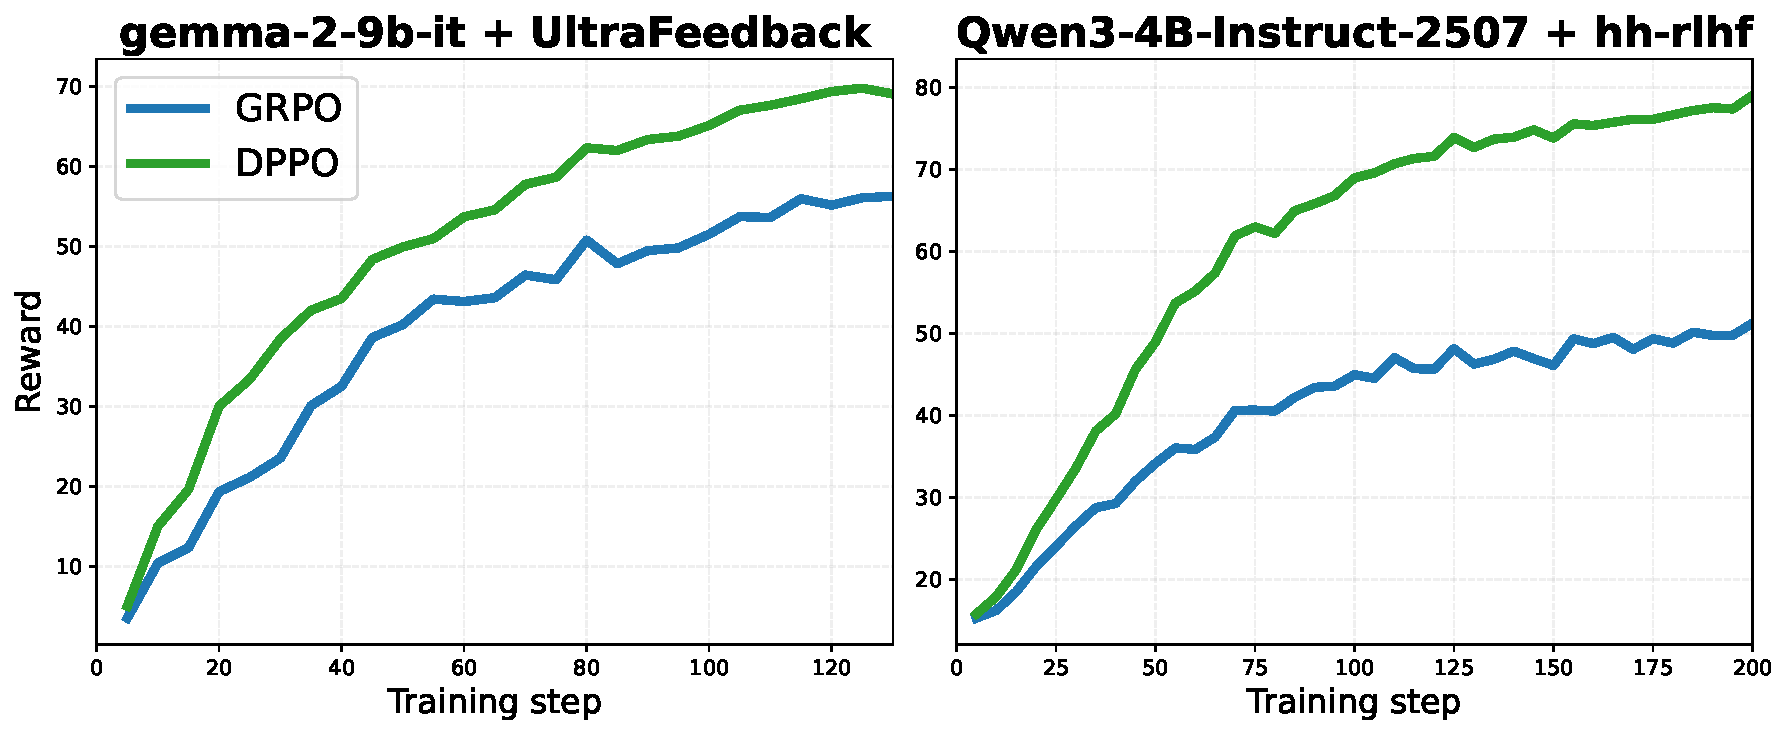
\includegraphics[width=1.0\linewidth]{figs/grpo_vs_dppo_more_rlhf.pdf}
    \caption{RLHF experiments with Skywork-Reward-Llama-3.1-8B as the reward model. DPPO improves reward faster and reaches higher final reward than GRPO on both Gemma-2-9B-It with UltraFeedback and Qwen3-4B-Instruct-2507 with HH-RLHF.}
    % \vspace{-0.4cm}
    \label{fig:more_rlhf}
\end{figure}

To evaluate DPPO beyond verifiable rewards, we further conduct RLHF experiments on open-ended alignment data. We compare GRPO with DPPO-Binary-TV in two settings: Gemma-2-9B-It~\citep{team2024gemma} trained on UltraFeedback~\citep{cui2023ultrafeedback}, and Qwen3-4B-Instruct-2507~\citep{yang2025qwen3} trained on HH-RLHF~\citep{bai2022training}. Both settings use Skywork-Reward-Llama-3.1-8B~\citep{liu2024skywork} as the reward model. As shown in \Cref{fig:more_rlhf}, DPPO improves the learned reward substantially faster and reaches higher final rewards in both settings. We further evaluate the fine-tuned Qwen3 models on AlpacaEval 2.0 in Appendix~\ref{appendix:rlhf_alpacaeval}, where DPPO achieves 80.90 length-controlled and 79.93 raw win rates, establishing a new SOTA on the \href{https://tatsu-lab.github.io/alpaca_eval/}{AlpacaEval 2.0 community leaderboard}. These results show that the effectiveness of DPPO also generalizes to noisy learned-reward optimization.


% \textbf{Ablation on TV/KL Approximation.}
\subsection{Ablation on Divergence Approximation}

\begin{figure}[h]
    \centering  
    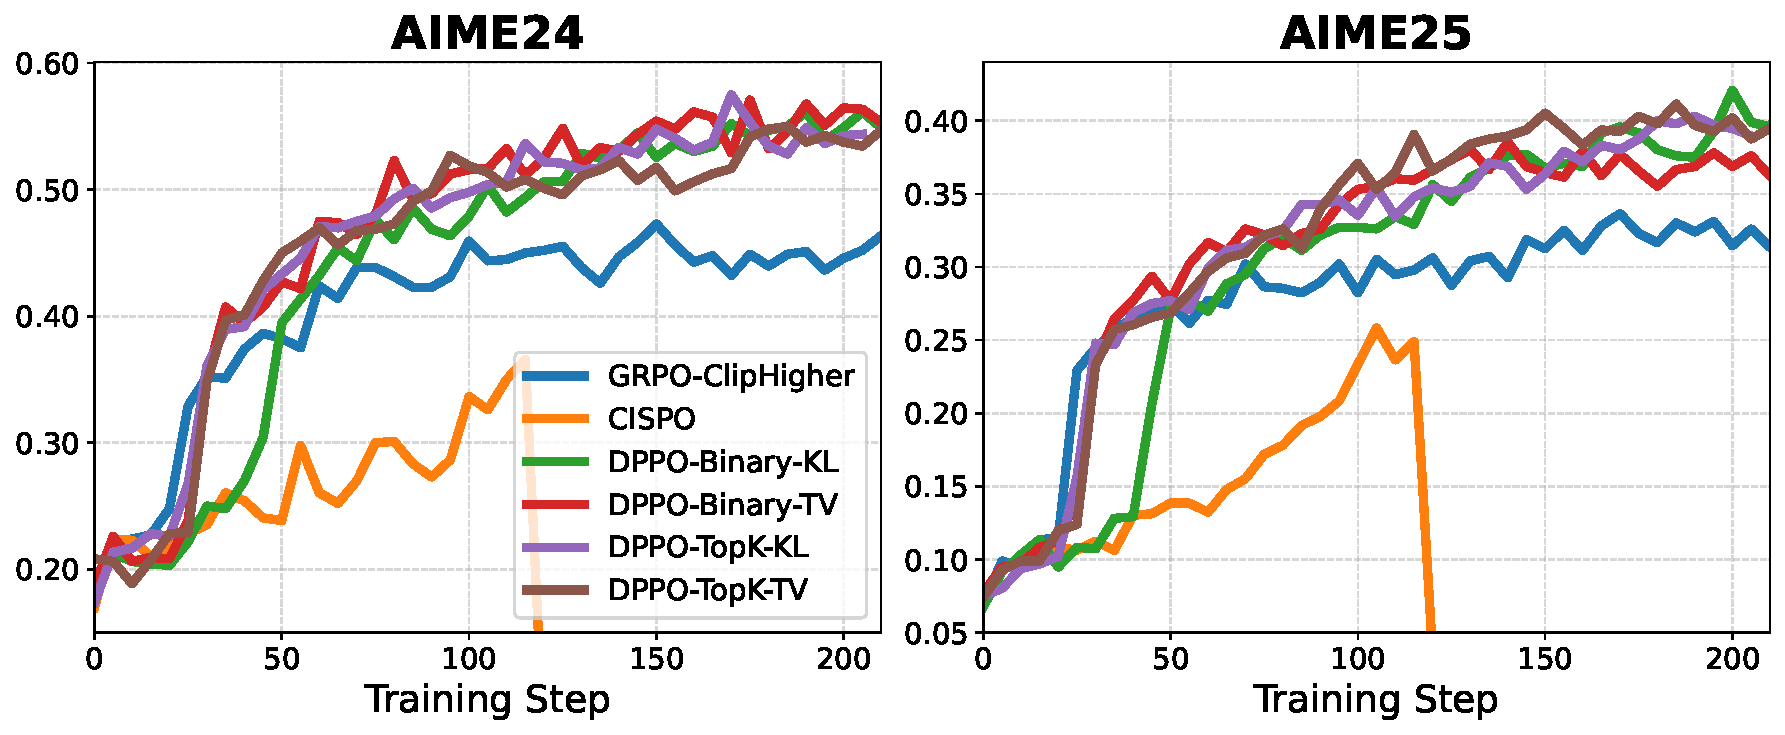
\includegraphics[width=1.0\linewidth]{figs/main-topk.pdf}  
    \caption{Evolution of AIME24 and AIME25 scores for baselines and DPPO with binary/Top-K (K=20) TV/KL approximation under the same setting as MoE Base w/o R3.}  
    \label{fig:main_topk}  
    % \vspace{-0.3cm}
\end{figure}

In the above experiments, DPPO is implemented using the binary TV/KL approximation (Equations~\ref{eq:binary_tv} and \ref{eq:binary_kl}). To assess the impact of this simplification, we compare it against DPPO with the top-K (K=20) TV/KL (Equations~\ref{eq:topk_tv} and \ref{eq:topk_kl}) under the same setting as MoE Base. The results, presented in \Cref{fig:main_topk}, show that both approximations perform similarly and significantly outperform the baselines. This finding indicates that the easy-to-implement binary approximation is a sufficient and computationally efficient choice for scalable RL. We provide more detailed results in Appendix~\ref{appendix:ablation_topk_approximation}.


% \begin{figure}[t]
%     \centering  
%     \includegraphics[width=1.0\linewidth]{figs/main-lora.pdf}  
%     \caption{Evolution of AIME24 and AIME25 scores during RL training with LoRA using Qwen3-30B-A3B-Base.}  
%     \label{fig:main_lora}  
%     % \vspace{-1.4em}
% \end{figure}



% \textbf{Generalization to Other Model Families and Tasks.}
\subsection{Generalization to Other Model Families and Tasks}
We also conduct experiments on Llama family models~\citep{touvron2023llama,wang2025octothinker} and on general reasoning tasks~\citep{liu2025gem}. The results, which are presented in Appendix ~\ref{appendix:extended_models_tasks}, show DPPO outperforms the baseline across most settings, highlighting its broad applicability.


% \textbf{Hyperparameter Sensitivity.}
\subsection{Hyperparameter Sensitivity}
We provide the hyperparameter sensitivity experiments in Appendix \ref{appendix:hyperparameter_sensitivity}.
